% Standalone TikZ block diagram of the PLASMC control pipeline.
% Compile:  pdflatex block_diagram.tex
%
\documentclass[tikz,border=3pt]{standalone}
\usepackage{amsmath}
\usepackage{amssymb}
\usepackage{bm}
\usetikzlibrary{arrows.meta,positioning,calc,fit,backgrounds,shapes.geometric}

\begin{document}
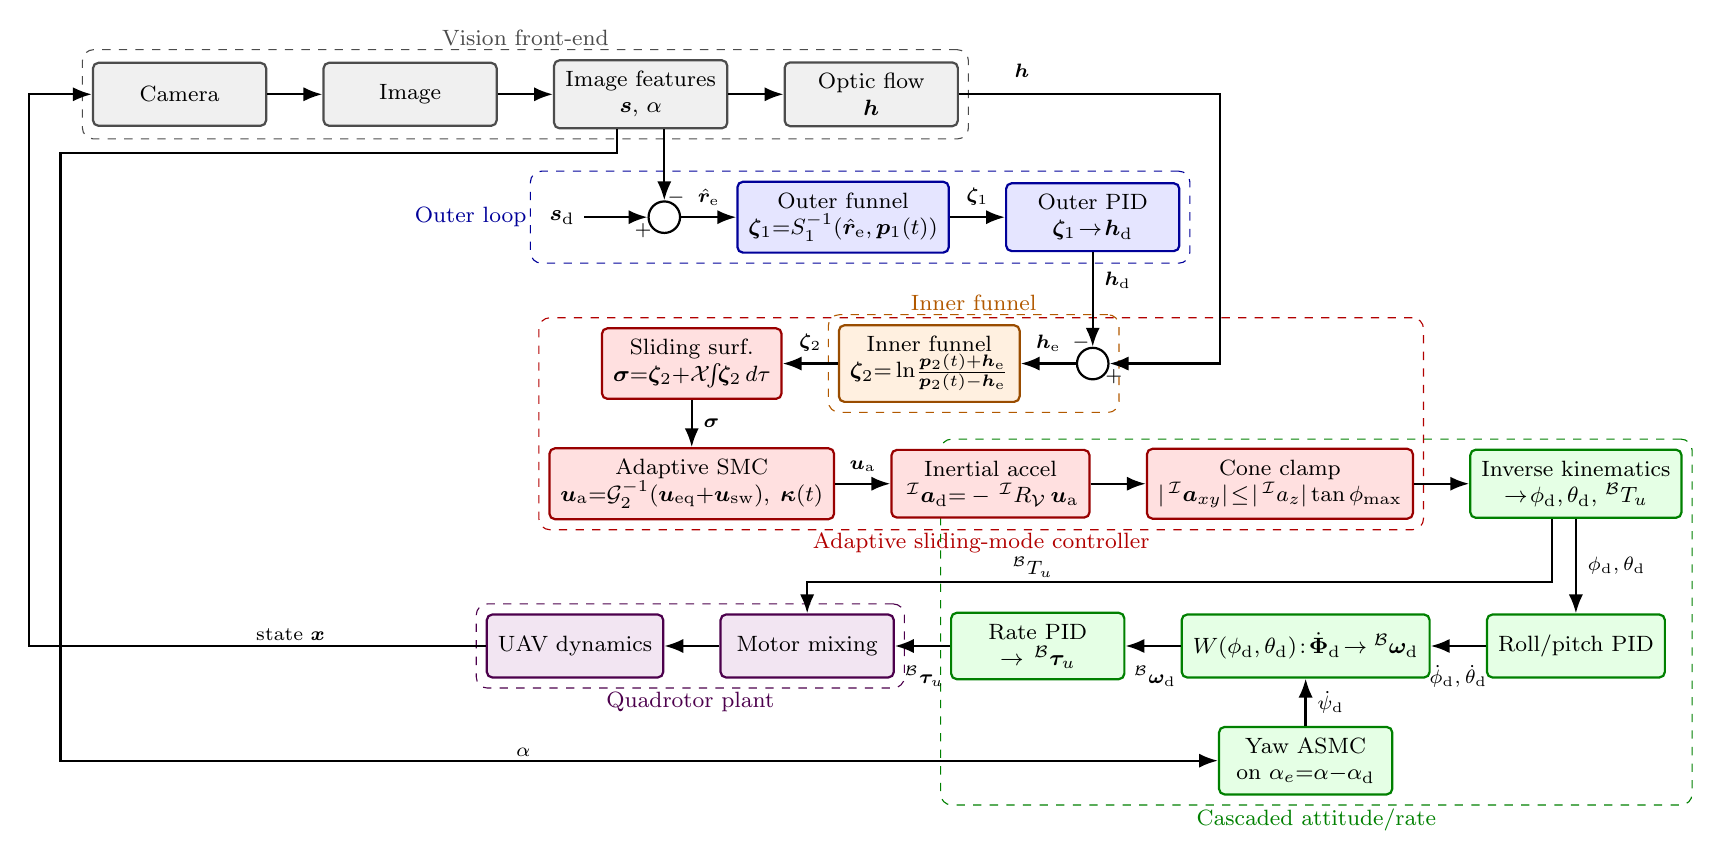
\begin{tikzpicture}[
    >=Latex,
    font=\footnotesize,
    node distance=5mm and 7mm,
    block/.style={
        rectangle, rounded corners=2pt, draw=black, thick,
        minimum height=8mm, minimum width=22mm,
        align=center, fill=white, inner sep=4pt
    },
    sens/.style ={block, fill=gray!12,   draw=gray!60!black},
    outer/.style={block, fill=blue!10,   draw=blue!60!black},
    inner/.style={block, fill=orange!12, draw=orange!60!black},
    asmc/.style ={block, fill=red!12,    draw=red!60!black},
    base/.style ={block, fill=green!10,  draw=green!50!black},
    plant/.style={block, fill=violet!10, draw=violet!60!black},
    sum/.style={
        circle, draw=black, thick, inner sep=0pt, minimum size=4mm,
        font=\scriptsize
    },
    flow/.style={->, thick, line width=0.3mm},
    edgelbl/.style={font=\scriptsize, inner sep=1pt},
    signlbl/.style={font=\scriptsize, inner sep=0pt},
    grouplbl/.style={font=\footnotesize, inner sep=1pt}
]

% =============================================================
% ROW 1 — Vision front-end
% =============================================================
\node[sens] (cam)   {Camera};
\node[sens, right=of cam]  (img)  {Image};
\node[sens, right=of img]  (feat) {Image features\\$\boldsymbol{s},\,\alpha$};
\node[sens, right=of feat] (vh)   {Optic flow\\$\boldsymbol{h}$};

% =============================================================
% ROW 2 — Outer (visibility) loop
% =============================================================
\node[sum,   below=9mm of feat, xshift=3mm] (e1)   {};
\node[outer, right=of e1]        (fnl1) {Outer funnel\\$\boldsymbol{\zeta}_1{=}S_1^{-1}(\hat{\boldsymbol{r}}_\text{e},\boldsymbol{p}_1(t))$};
\node[outer, right=of fnl1]      (pid)  {Outer PID\\$\boldsymbol{\zeta}_1\!\to\!\boldsymbol{h}_\text{d}$};
\node[left=8mm of e1] (sd) {$\boldsymbol{s}_\text{d}$};

% =============================================================
% ROW 3 — Inner (optic-flow) loop
% =============================================================
\node[sum,   below=12mm of pid]  (e2)   {};
\node[inner, left=of e2]         (fnl2) {Inner funnel\\$\boldsymbol{\zeta}_2{=}\ln\!\frac{\boldsymbol{p}_2(t){+}\boldsymbol{h}_\text{e}}{\boldsymbol{p}_2(t){-}\boldsymbol{h}_\text{e}}$};
\node[asmc,  left=of fnl2]       (sld)  {Sliding surf.\\$\boldsymbol{\sigma}{=}\boldsymbol{\zeta}_2{+}\mathcal{X}\!\!\int\!\!\boldsymbol{\zeta}_2\,d\tau$};

% =============================================================
% ROW 4 — Adaptive SMC chain
% =============================================================
\node[asmc,  below=6mm of sld]  (asmc) {Adaptive SMC\\$\boldsymbol{u}_\text{a}{=}\mathcal{G}_2^{-1}(\boldsymbol{u}_{\text{eq}}{+}\boldsymbol{u}_{\text{sw}}),\;\boldsymbol{\kappa}(t)$};
\node[asmc,  right=of asmc]      (iacd) {Inertial accel\\$\,^\mathcal{I}\boldsymbol{a}_\text{d}{=}-\,^\mathcal{I}R_\mathcal{V}\,\boldsymbol{u}_\text{a}$};
\node[asmc,  right=of iacd]      (cone) {Cone clamp\\$|\,^\mathcal{I}\boldsymbol{a}_{xy}|\!\le\!|\,^\mathcal{I}a_z|\tan\phi_{\max}$};
\node[base,  right=of cone]      (ik)   {Inverse kinematics\\$\to\!\phi_\text{d},\theta_\text{d},\,^\mathcal{B}T_u$};

% =============================================================
% ROW 5 — Horizontal attitude/rate cascade below ASMC row.
% 12mm gap leaves room for the ASMC group label + T_u bypass.
% =============================================================
\node[base,  below=12mm of ik]   (att)  {Roll/pitch PID};
\node[base,  left=of att]        (mux)  {$W(\phi_\text{d},\theta_\text{d})\!:\!\dot{\boldsymbol{\Phi}}_\text{d}\!\to\!\,^\mathcal{B}\boldsymbol{\omega}_\text{d}$};
\node[base,  left=of mux]        (rpid) {Rate PID\\$\to\,^\mathcal{B}\boldsymbol{\tau}_u$};
\node[plant, left=of rpid]       (mix)  {Motor mixing};
\node[plant, left=of mix]        (uav)  {UAV dynamics};

% Yaw ASMC
\node[base,  below=6mm of mux]   (yaw)  {Yaw ASMC\\on $\alpha_e{=}\alpha{-}\alpha_\text{d}$};

% =============================================================
% CONNECTIONS — every label offset 1–2mm from its arrow
% =============================================================

% Vision chain
\draw[flow] (cam)  -- (img);
\draw[flow] (img)  -- (feat);
\draw[flow] (feat) -- (vh);

% --- Outer loop ---
\draw[flow] (sd) -- (e1);
\draw[flow] ([xshift=3mm]feat.south) -- (e1.north);
% +/- placed as standalone nodes at fixed offsets from the sum circle
\node[signlbl] at ([xshift=-2.7mm, yshift=-1.7mm]e1) {$+$};
\node[signlbl] at ([xshift=1.5mm, yshift=2.5mm]e1) {$-$};

\draw[flow] (e1)   -- (fnl1) node[edgelbl, midway, above, yshift=1mm]{$\hat{\boldsymbol{r}}_\text{e}$};
\draw[flow] (fnl1) -- (pid)  node[edgelbl, midway, above, yshift=1mm]{$\boldsymbol{\zeta}_1$};

% --- Inner loop ---
\draw[flow] (pid.south) -- (e2.north)
    node[edgelbl, pos=0.30, right, xshift=1mm]{$\boldsymbol{h}_\text{d}$};

% h wraps RIGHT of pid and enters e2 from EAST
\draw[flow] (vh.east) -| ([xshift=5mm]pid.east |- e2.east) |- (e2.east);
% h label on the horizontal leaving vh (separate draw for clean placement)
\node[edgelbl] at ([xshift=8mm, yshift=3mm]vh.east) {$\boldsymbol{h}$};

% +/- on e2 as standalone nodes
\node[signlbl] at ([xshift=-1.5mm, yshift=2.7mm]e2) {$-$};
\node[signlbl] at ([xshift=2.7mm, yshift=-1.7mm]e2) {$+$};

\draw[flow] (e2)   -- (fnl2) node[edgelbl, midway, above, yshift=1mm]{$\boldsymbol{h}_\text{e}$};
\draw[flow] (fnl2) -- (sld)  node[edgelbl, midway, above, yshift=1mm]{$\boldsymbol{\zeta}_2$};

% --- ASMC chain ---
\draw[flow] (sld)  -- (asmc) node[edgelbl, midway, right, xshift=1mm]{$\boldsymbol{\sigma}$};
\draw[flow] (asmc) -- (iacd) node[edgelbl, midway, above, yshift=1mm]{$\boldsymbol{u}_\text{a}$};
\draw[flow] (iacd) -- (cone);
\draw[flow] (cone) -- (ik);

% --- Horizontal attitude/rate cascade (right to left) ---
\draw[flow] (ik) -- (att) node[edgelbl, midway, right, xshift=1mm]{$\phi_\text{d},\theta_\text{d}$};
\draw[flow] (att) -- (mux) node[edgelbl, midway, below, yshift=-2mm]{$\dot{\phi}_\text{d},\dot{\theta}_\text{d}$};
\draw[flow] (yaw.north) -- (mux.south) node[edgelbl, midway, right, xshift=1mm]{$\dot{\psi}_\text{d}$};
\draw[flow] (mux)  -- (rpid) node[edgelbl, midway, below, yshift=-2mm]{$\,^\mathcal{B}\boldsymbol{\omega}_\text{d}$};
\draw[flow] (rpid) -- (mix)  node[edgelbl, midway, below, yshift=-2mm]{$\,^\mathcal{B}\boldsymbol{\tau}_u$};
\draw[flow] (mix)  -- (uav);

% T_u bypass from IK → mix
\draw[flow] ([xshift=-3mm]ik.south) -- ++(0,-8mm) -| (mix.north)
    node[edgelbl, pos=0.35, above, yshift=0.05mm]{$\,^\mathcal{B}T_u$};

% State feedback wraparound: enter cam from WEST.
% Label placed as standalone node to the left of UAV dynamics.
\draw[flow] (uav.west) -- ++(-6mm,0)
    -| ([xshift=-8mm]cam.west) |- (cam.west);
\node[edgelbl, left=20mm of uav.west, yshift=4.0, anchor=east] {state $\boldsymbol{x}$};

% α feed from image features to Yaw ASMC.
\draw[flow] ([xshift=-3mm]feat.south) -- ++(0,-3mm)
    -| ([xshift=-4mm]cam.west |- yaw.west) -- (yaw.west)
    node[edgelbl, pos=0.4, above]{$\alpha$};

% =============================================================
% Group backdrops
% =============================================================
\begin{pgfonlayer}{background}
  \node[draw=gray!60!black, dashed, rounded corners,
        fit=(cam)(img)(feat)(vh),
        inner sep=1.2mm,
        label={[grouplbl, gray!60!black]above:Vision front-end}] {};
  \node[draw=blue!60!black, dashed, rounded corners,
        fit=(sd)(e1)(fnl1)(pid),
        inner sep=1.2mm,
        label={[grouplbl, blue!60!black]left:Outer loop}] {};
  \node[draw=orange!70!black, dashed, rounded corners,
        fit=(e2)(fnl2),
        inner sep=1.2mm,
        label={[grouplbl, orange!70!black]above:Inner funnel}] {};
  \node[draw=red!70!black, dashed, rounded corners,
        fit=(sld)(asmc)(iacd)(cone),
        inner sep=1.2mm,
        label={[grouplbl, red!70!black]below:Adaptive sliding-mode controller}] {};
  \node[draw=green!50!black, dashed, rounded corners,
        fit=(ik)(att)(mux)(rpid)(yaw),
        inner sep=1.2mm,
        label={[grouplbl, green!50!black]below:Cascaded attitude/rate}] {};
  \node[draw=violet!60!black, dashed, rounded corners,
        fit=(mix)(uav),
        inner sep=1.2mm,
        label={[grouplbl, violet!60!black]below:Quadrotor plant}] {};
\end{pgfonlayer}

\end{tikzpicture}
\end{document}
